\chapter{Implementation details}\label{chap:chap3}

\section{Outline}

As we have seen in Chapters \ref{chap:intro} and \ref{chap:sota}, there is a
rising awareness of the power of ML methods. PPLs, despite still being mostly
unknown to data scientists, provide an interface for defining personalized
probabilistic models and possess a built-in inference engine.
The benefits of VPLs when compared to a textual format are well-known, but there
is no VPL applied to a PPL, so we aim to create one.

A big requirement we wished to fulfill was, not only ease of use, but also ease
of installation. This means having portability across operating systems as well
as being able to execute without installing dependencies. For this reason, we
decided our VPE should run in the browser.

It was also important that we chose
a target PPL for which there is a decent amount of programs written on it, so we
could thoroughly test our hypothesis. Because it was the one
that best matched this criteria we chose Infer.NET to work with, a framework that
can be used in CLI languages (such as C#, F# or C++). Because none of these
languages can, at least at the time of writing (that might change when WebAssembly
\cite{weba} gets widespread support), be directly compiled to JavaScript
we will be sacrificing immediate
visual feedback and build a hybrid text and visual system (a VPE) rather than a purely
visual language (see Section \ref{sec:vpe} for more details). This means that
our tool won't be able to run the model the user defines, but will generate
Infer.NET (hosted in C#) code (see Figure \ref{fig:scope}).

The user can take the generated
code and run it in a separate runtime (such as CLR). While not the ideal scenario, because it
complicates the development and debugging cycles (in order to see each change,
users must first copy the code to a file in a machine that can compile and run it),
it has the advantage of seamlessly integrating with larger projects. An example
would be an enterprise application written in C# that has a small component
that the team who's developing it feels it would make sense to use a PPL there.
They can use our VPE to develop that portion of the program, and then just place
the code in the desired place. Using a purely visual programming language in the
same scenario, despite having a faster development time, would then require
a rewriting in a textual form.

\begin{figure}[t]
  \begin{center}
    \leavevmode
    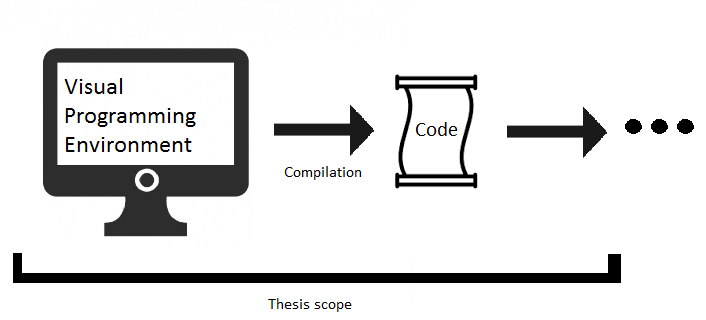
\includegraphics[width=0.86\textwidth]{scope}
    \caption{High-level look into our tool}}
    \label{fig:scope}
  \end{center}
\end{figure}

\section{Architecture}

 % "controlled dataflow vpl"
 In this section we will be explaining why we made certain choices, such as for
 the target PPL, the front-end framework or what features to include or not.

\section{Picking a target PPL}
\label{sec:tarppl}

Perhaps one of the most important decisions we had to made concerns the PPL we
would be offering a VPE to, since the visual programming concepts applied are
highly dependent on the language's own capabilities. For instances, we cannot
study how VP can be helpful in an object-oriented design if we are using a
purely functional PPL such as Church which does no have that concept.

As we seen on Section \ref{sec:ppls}, the PPL landscape is heterogeneous enough
that we could pick a language from any paradigm or runtime we wanted to, as there
are many alternatives available. So we could narrow down the scope, we decided to avoid
purely functional and logical programming languages, because we wanted to build
a VPE that was not an end in itself: meaning that it was not only useful to build
PP but also to help our target audience eventually transition from a graphical
environment to the textual form (or, at least, be able to use both if they need
a more fine-grained control in a certain scenario). Even if it is a matter of
debate which paradigm is more suitable to people learning how to program, we feel
that because imperative and object-oriented are more common in data science (the prime
examples being Python and R), they would be a better choice.

After applying this restriction, there were still many PPLs to chose from, so
we decided upon the main criteria on which to make our decision: the language
should have comprehensible and extensive documentation, plenty of code examples
with a variety of complexities, an active and helpful community, be hosted in
a mainstream programming language (as opposed to being a standalone language by itself)
and it should run on the browser. The first three points are related to how well
can we learn the language well enough to design a VPE for it, having no prior
experience with it, in a short amount of time. Being executable on the browser
would allow to provide instant visual feedback of the results, since the VPE
would not be limited to defining a model, but it would could execute it.

On a technical side the strongest candidate is VentureScript \cite{probcomp},
due to the fact it is hosted in javascript (with the aforementioned advantages).
Despite this advantage, it is still on Alpha and both the code examples and
documentation are still scarce, even taking into consideration its predecessor's
examples \cite{forestdb} and tutorials \cite{church}.

The three stronger candidates, after some selection, were PyMC \cite{pymc},
Figaro \cite{figaro} and Infer.NET \cite{InferNET14}. All three are hosted in popular languages
(Python, Scala and C#/F#, respectively) and have comprehensive tutorials and
documentation available \cite{pymct}\cite{figarot}\cite{InferNET14t}.

We ended up choosing Infer.NET because it had the widest range of examples
available, which is pivotal to design a VPE as complete as possible, as well
as evaluate it under different scenarios. Besides its complete documentation
and tutorial, its website features more than 20 code examples, as well as a list
of papers that resorted to Infer.NET. Some of these papers are about PP or PPL theory,
but others are about applications of it, such as "Automatic analysis and
identification of verbal aggression and abusive behaviors for online social
games" \cite{balci2015automatic}, which gives us confidence that Infer.NET is
mature enough so we can focus in the VPE design rather than struggling with
learning the language. Bottom line, it was chosen due to the abundant number of
programs written on it publicly available.

\section{Picking a front-end}

After knowing which would be the language we would be targeting, there was still
the need to define both the visual paradigm and the framework, if any, that we
would use to develop the front-end (visual interface) of our VPE.

Regarding the paradigms the two competing alternatives are VDP and the one offered
by Blockly. While the first approach is what we typically see in similar tools,
such as RapidMiner or NoFlo, the second one is a fairly new approach, unseen
in tools other than those which were built using Blockly. It is not trivial to
assess the suitability of either of the options because there was never a study
directly comparing the merits of each of them, so we will try to make our own
analysis by comparing their strenghts and weaknesses while assessing what is
more valuable in the context of a VPE for a PPL.

\subsubsection{Blockly}
\label{sec:fblock}

Similarly to what happens with VP and VPEs, there are plenty of references
in the literature that Blockly-based tools boost productivity \cite{Marron2012} and ease the process
of learning how to program \cite{Junior2006}.

When compared with tools that are
based in a VDP approach, it has a representation that is more similar to how code
is written \cite{blockly}, which can be an advantage in a tool that aims to serve as a visual
interface that generates code in a textual format, such as the one we're developing.
This can be seen as an advantage because, not only does it facilitate fully transitioning
to a textual format as soon as the user is comfortable enough at programming,
but it is also makes it easier to textually fine-tune a code that was developed
using the VPE.

Among the features we analyzed in Section \ref{sec:sotavdp} that deal with
helping the user achieving program correction we saw syntax checking and type
checking. Blockly addresses both situations by visually modeling the program
as a puzzle where only compatible pieces fit together; this is an intuitive way
to enforce correctness, since it maps to an activity the majority of people are
familiarized with: assembling puzzles. This seems a better way to cope with errors
rather than showing an error message at compile or run-time, because often it is
not even clear that there is an error, as we have seen that happens with NoFlo in
Section \ref{sec:noflo}.

Another great advantage of Blockly is that, because it runs on the browser, it is
compatible across devices and operating while not requiring any kind of setup.
If the user choses to download Blockly, it can even work with it without internet
connection. The same applies to our VPE if we chose to build it on top of Blockly.

However, this VPE of VPEs lacks features that enable it to effectively scale up
such as the ones we have seen with NoFlo or Blender Composite Nodes (Section \ref{sec:sotavdp}).
Examples of this include being able to zoom in and out in the UI, searching for
blocks by their name, zoom in and out or create group blocks to encapsulate a certain group of
nodes (a concept analogous to functions in regular programming). It enables the
creation of vertically and horizontally compressed blocks, similarly to Viskell,
by using block composition and dropdowns rather than requiring to plug-in extra blocks
(see Figure \ref{fig:blocklycomp} for an example of each case).

\begin{figure}[t]
  \begin{center}
    \leavevmode
    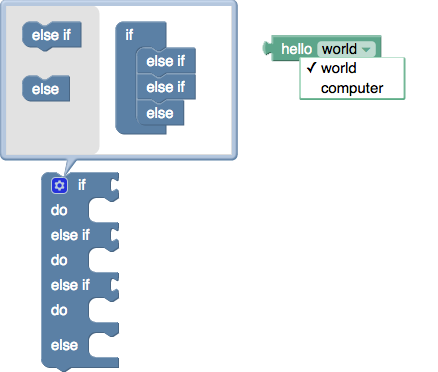
\includegraphics[width=0.86\textwidth]{blocklycomp}
    \caption{Blockly example of horizontal and vertical compression \cite{blockly}}
    \label{fig:blocklycomp}
  \end{center}
\end{figure}

\subsubsection{Eclipse Toolset}

The Eclipse Foundation has some tools, which are accessible as plugins for the
Eclipse IDE, that we thought that could serve as a foundation for the VPE we're
aiming to develop.

Damos \cite{damos}, a project still in the "Proposal" phase of the Eclipse
Development Process, is a framework for building data-flow graphical languages
and their respective code generator. It includes both graphical and textual editors,
as well as support for continuous, synchronous and asynchronous computations.
Even if it already includes enough blocks so it can be used by engineers and scientists
as a replacement for tools like MATLAB/Simulink or LabVIEW, it was designed to
be customizable and extensible with new blocks, so we could use it to build our VPE on.

Damos uses another Eclipse tool as its graphical editor: the Graphical Modeling
Framework (GMF). GMF can be used to build graphical editors for multiple visual
languages \cite{gmf}, such as UML modeling, application interfaces such as the
one described in Section \ref{sec:winb} or, eventually, a visual language for a
PPL. GMF is often used in conjunction with the Eclipse Modeling Framework (EMF),
"a modeling framework and code generation facility for building tools and other
applications based on a structured data model" \cite{emf}.

In spite of their advantages, all of these have two common problems. First, they require
users to download both Eclipse and the used plugins and their dependencies
which not only constitutes an entry barrier but hinders collaboration, because
it makes it difficult to share the model among colleagues. And secondly, they
were built to generate code to specific target languages (C for Damos and Java
for EMF), neither of which has a PPL implementation with a strong community
(Probabilistic-C \cite{Paige2014} serves as a proof of concept and we already explained
in Section \ref{sec:tarppl} why we discarded Figaro). Even if we could eventually
use the generated C or Java as an intermediary representation, we believe the
extra burden (both in development time and in runtime performance) of having an
extra transformation does not justify for the added benefits when compared with
other front-ends.

\subsubsection{Custom implementation}

At this point the strongest candidate for a front-end was Blockly,
but it would also be possible to fully develop a new front-end, instead of using
a framework such as Blockly or the tools from the Eclipse toolset. The purpose of
doing so would be overcoming Blockly's limitations that we refered earlier in
Section \ref{sec:fblock}. In order to keep Blockly's portability, we would have an
implementation targeting the browser, where the visual elements would be
represented by DOM tree elements and drawn using the browser's render engine,
just like a regular HTML page; for performance reasons, we could use the HTML
\textit{canvas} element \cite{w3ccanvas}.

The reason why we won't be choosing this option is that we believe that this
flexibility of implementing extra features, that essentially have to do with
navigation and block filtering or selection, are not worth the risk of having
a VPE that does not feel as fluid and as natural as Blockly or GMF implementation would, since all
those aforementioned features are secondary when compared to the look and feel
of the core VPE (by core we mean the workspace where we drag the blocks, edit
their inline properties and connect them).

Examples of such core usability features, besides having a layout that has already been
tested (proven to deliver the benefits of VP)
that Blockly already provides include magnetic connections
(you don't have to drag and drop a block to a stricly defined area, doing so near
a valid connection highlights that connection and makes it possible to drop it there)
and block mutations (a block may change when you connect certain blocks to it,
this allows for horizontal and vertical compression).

Using a third-party framework also has the advantage of automatically getting new
features as soon as that framework is updated, such as the zoom in and out that
Blockly is planning to deliver \cite{blockly}.

\section{Development steps}

The purpose of this section is to enumerate the difficulties encountered when
developing a VPE that could support the design of programs similar in functionality
to the ones the reader can find in Infer.NET's tutorials \cite{InferNET14t} and
the solution we adopted to overcome them.

\subsection{Generating basic C#}

Since Infer.NET is hosted in C# but Blockly does not include a generator for
the language, the first thing to do was to be able to provide code generation for
Blockly's default blocks, that provide a language's most basic constructs such
as variables, lists and control structures.

We decided to adopt an open-source implementation to solve this issue \cite{csgen}
but since it was not compatible with Blockly's versions since January 2016, it
was necessary to work on making it compatible, so we could have the latest features
available, such as zooming in and out, which we had previously identified as a
major feature required in a VPE to be able to scale up programs visually.

This work lead to the pull request \#8 to that open-source project \cite{csgenpr}.

\subsection{Mandatory declarations}

Similarly to Java and C/C++, in order to run a program, you must provide a method
as an entry point, where the control flow will start and end. However, a textual
representation generated by Blockly does not comtemplate this possibility, so
we had to figure out how to deal with this issue. Figure \ref{fig:before} shows a simple program,
and this is its generated code:

\begin{figure}[t]
  \begin{center}
    \leavevmode
    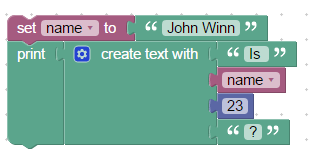
\includegraphics[width=0.86\textwidth]{before}
    \caption{Blockly simple example}
    \label{fig:before}
  \end{center}
\end{figure}

\begin{lstlisting}
dynamic name;


name = "John Winn";
Console.WriteLine(String.Concat("Is ", name, 23, "?"));
\end{lstlisting}

If you try to run this code you will get a compile-time error, as expected.

Another issue that arises when representing Infer.NET programs in Blockly is how
to specify inference engine settings, such as the algorithm is should use, if it
parallelizes for-loops, if it re-allocates internal messages between inference
runs, etc. Unlike other kinds of statements, such as loops, variable declarations
or prints, these settings are usually only set once per program and remain
unaltered.

Having both these situations in mind, a possible solution is to use a singleton
block (one that must be present in every representation and can't be deleted),
where we aggregate both these concerns and which contains the remainder of the program.
Such an example can be seen in Figure \ref{fig:after}, which generates the following code:

\begin{figure}[t]
  \begin{center}
    \leavevmode
    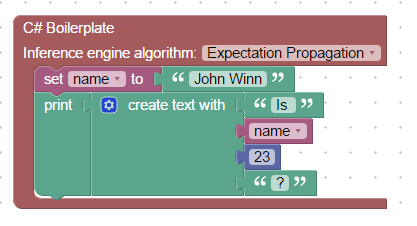
\includegraphics[width=0.86\textwidth]{after}
    \caption{Blockly simple example with C# boilerplate}
    \label{fig:after}
  \end{center}
\end{figure}

\begin{lstlisting}
using System;
using System.Collections.Generic;
using System.Text;
using MicrosoftResearch.Infer.Models;
using MicrosoftResearch.Infer;

namespace InferBlockly
{
	public class InferBlockly
	{
		public void Run()
		{
			InferenceEngine engine = new InferenceEngine();
			engine.Algorithm = new ExpectationPropagation();
			dynamic name;


			name = "John Winn";
			Console.WriteLine(String.Concat("Is ", name, 23, "?"));
		}
	}
}
\end{lstlisting}

Despite losing flexibility, since it is impossible to change the settings
throughout the program (even if that is valid in Infer.NET),
we believe that this increased simplicity is more intuitive and therefore benefitial to an unexperienced
programmer than allowing the settings to be changed at any point in time.

\subsection{Variable type checking}

Every PPL has the concept of random variables, which are the building block of
any PP. Some examples in Infer.NET are listed below.

\begin{lstlisting}
  			Variable<bool> firstCoin = Variable.Bernoulli(0.5);
        Variable<double> x = Variable.GaussianFromMeanAndVariance(0, 1);
        Variable<double> threshold = Variable.New<double>();
        Variable<double> precision = Variable.GammaFromShapeAndScale(1, 1);
        VariableArray<double> x = Variable.Array<double>(dataRange);
        VariableArray<bool> y = Variable.Observed(willBuy);
\end{lstlisting}

Because there are so many different types (we are showing 4, but there are more),
we believe our VPE should help the user avoid mistakes related with using wrong
types, such as trying to apply logical operators to numeric random variables or
greater than comparisons between boolean variables.

When choosing how to represent variables we had to take into account that
Blockly was conceived to target dynamic languages, as it can be seen by the languages
it targets: JavaScript, Python, PHP and Dart (which supports static type-checking,
but it's not the default mode \cite{dart}). The negative consequence of this is that it's
not ready to perform type checking on variables, meaning that an user can
produce invalid programs when using variables (as seen in Figure \ref{fig:valid_blockly}, we have
drawn a program that will produce a runtime exception, since we can't evalaute
the square root of a text string), althought the same doesn't happen when
directly connecting the blocks, since we can't connect text input blocks to the
right connector of the square root block.

There have been dicussions among open-source projects that rely on Blockly on how
to incorporate type checking for variables (such as a VPE for Arduino \cite{bduino}
or one for Kiwi.js \cite{gbl}, an HTML5 game framework) as well as in Blockly's
dicussion forum \cite{gbl2}, but none reached a final proposal, let along a working
implementation.

Therefore, we have decided to extend Blockly in order to be able to support
different types of variables with a similar type check to the one used in other
kinds of blocks, meaning that if they don't type check, the pieces don't fit and the user
can't connect them. This was done by adding an extra field to FieldVariable
(the class Blockly class that represents variables) that identifies its type and
modifying the behavior of each component that deals with variables to take that
into account \footnote{These changes can be found in github.com/gcandal/blockly/commit/8f5fa0}.

This way, variables from different types are kept isolated, so that if the user
declares a boolean variable named \textit{bool}, it won't appear in numeric
variable's dropdowns or menus. This segregation between different variable types,
besides allowing to have the aforementioned type checking at the block level, it
also allows to have different colors and labels in the blocks for different types of variables
(making it clearer to the user they should be used differently) and to declare
explicit C# types in the generated code, rather than using
the dynamic keyword to avoid static type-checking \cite{cdyn}. The advantage is that
the generated code is closer to the one that would be written by a programmer,
so it eases the transition from a VPE to a textual format, since both representations
are similar.

\begin{figure}[t]
  \begin{center}
    \leavevmode
    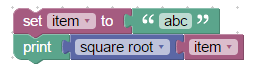
\includegraphics[width=0.86\textwidth]{valid_blockly}
    \caption{Blockly example of representable invalid program}
    \label{fig:valid_blockly}
  \end{center}
\end{figure}

\subsection{Serialization}

It is important in a VPE to be able to save and load programs, so the user can
not only work on a given program at different points in time, but also share it
with other users. Blockly makes it possible to do so by converting a graphical
representation to XML, which can later be imported.

We have extended Blockly so this functionality could be easily acessible in the
GUI, and the XML can be saved and loaded into the computer that's running the VPE.

\subsection{Remote execution}

\section{Limitations}

In this section we will describe some limitations that our chosen toolset (using
Blockly to represent Infer.NET C#) imposes in functionality.

\subsection{Inverse compilation}

By inverse compilation we mean the act of converting a program in a textual form
to its Blockly representation. This could be useful because it would help users
easily switch between representations, similarly to Window Builder (as discussed in Section \ref{sec:winb})
and unlike what happens with our current approach.
With our VPE, if you textually make a change in the the program by directly
writing in the text-area where ir appears,
and since that won't be reflected in the graphical representation, everytime
the code is re-generated (which happens frequently and unexpectedly, in situations
such as opening and closing menu tabs) your changes will be overriden.

Even if parsing C# and converting it to an intermediate representation would be
simple (Microsoft provides an EBNF grammar for the language \cite{ebnfcs}), there
are a number of questions that should be explored before implementing this feature.
For instances, our graphical representation guarantees type safety and a valid
program so it would not make sense to allow specifying an invalid program that
would be translated into a graphical form, it would break one of the most important
guarantess, the one that makes it suitable for beginners in programming. In
order to ensure a valid textual program, we would need to be able to either mimick
the compiler's verifications or run the compiler itself; the first option is
a big challenge while the second still requires further investigation on how
to handle users' errors.

\subsection{Instant visual results}

As we discussed before in several parts of this work, a big tradeoff we made was
to sacrifice the flexibility of using any language needed in favor of the portability
of a VPE that runs in the browser, which (as of this moment) only runs JavaScript.

Perhaps the greatest limitation of this approach is not being able to run Infer.NET
code, which makes it impossible not to violate the VP principle of instant visual results.
The development cycle is greatly affected by forcing the user to copy the text
into a location where a compiler can access and run it. A work around for this
is to adopt a client-server architecture where our server would run the code
and send the results back to the user. Even if that creates a need for internet
connection, which currently does not exist, we believe it to be a worthwhile tradeoff
and so we have chosen to implement it.

The downside of this approach is that we have to wait for the round-trip time
of the program to be sent to the server plus the compilation and execution times.
During this process, the user does not get any feedback; this could be minimized
by providing push notifications to the client and streaming the program's output,
rather than waiting for the execution to finish to get a response.

\subsection{Object-oriented programming}

You may notice that, even while we're targeting an object-oriented programming
language, our VPE has no support for representing classes. It also does not
support file management (splitting the program in several files) or namespaces.

The reason for this is that our target audience is not concerned with those features.
As discussed in Section \ref{sec:vp} VP is best suited for small domains, and our
VPE is meant to help data scientists and statisticians with little or no programming
experience start getting familiar with PP through a PPL, and not provide a
fully featured IDE.

Incorporating this kind of features, although feasible, would significantly
make the VPE more complex both in terms of cluttering the interface and the user
experience by providing mostly unecessary options, thus having little added
benefit to the majority of users.

\section{Tutorial}

\section{Conclusions}
